
In order to validate the DAL it was designed a way to simulate a crowd, that allows us to run multiple experiments with large datasets in a viable time and without the possible biasing issues that can occur when using a human crowd. The solution found was to create the Crowd Simulator, a parameterized system that can simulate crowds with different levels of reliability, providing many contributions in short time.

To determine how the Crowd Simulator should work, we had to understand the behavior of the crowd. Yu et al.\cite{yu2012challenges} classify the crowd in four categories: Hon workers: honest worker agents who return high quality HIT (human intelligence task) results randomly 90\% of the time; MH workers: moderately honest worker agents who return high quality HIT results randomly 70\% of the time; MM workers: moderately malicious worker agents who return high quality HIT results randomly 30\% of the time; Mal workers: malicious worker agents who return high quality HIT results randomly 10\% of the time. In our scenario we consider a high quality HIT as a positive synchronization point identification or correct negation.

Per these definitions, the Crowd Simulator is settled with the percentage of honest workers in the simulated crowd, and we name this parameter as Crowd Trustworthy Degree. Each time the simulator is called, it determines the current worker reliability as so the chance of his contribution represents a high quality answer. As the objective of this experiment is validating de DAL, each high quality result is extracted from a Gold Standard Table that contains all relations between videos in dataset.

For this experiment we used the Climbing video dataset \cite{hal-01162603} that contains 89 videos captured from several different devices and users in order to register a climbing activity by distinct points of view. This climbing event has 4327.3 seconds long, and the videos starts in different offsets with durations varying between 18.96 and 1259.06 seconds. We made tests for 11 Crowd Trustworthy Degrees (from 100\% to 0\%) running 30 full simulations for each degree. Table 1 presents, for each Crowd Trustworthy Degree, the median of how many contributions were needed to converge the DAL (find all time offsets) after 30 roll of the simulation, the number of relations found, and the error rate.

As the dataset contains 89 videos, the goal was to find all 3916 relations for all pairs of videos in it. To reduce the false convergences, we used the convergence level three to determine that a value is assumed correct, this means that at least three sequential agreements are necessary to converge a value.

We also created a Gold Standard DAL built with 100\% of correct answers from de Gold Standard Table (available with the dataset), allowing us to compare the DAL generated in each run with the Gold Standard DAL for accuracy and efficiency of the simulated crowd.  Table~\ref{xp1} shows the results of the simulation. Each line corresponds to a test with different Trustworthy Degrees (reliability).  Besides the reliability, each line presents the number of necessary contributions to converge, the total amount of possible relations (not all relations will present values, as there may be GAPs among videos) found among pairs of videos and the error degree.


\begin{table}
\begin{center}
\caption{Median for all 89 Videos, after 30 rolls of simulations for each Trustworthy degree} \label{xp1}
\begin{tabular}{|c|c|c|c|}
  \hline
  Reliability & Contributions & Relations & Error
  \\
  \hline
  100\% & 11161 & 1115 & 9\% \\
  90\%  & 12101 & 1095 & 10\% \\
  80\%  & 13199 & 1095 & 10\% \\
  70\%  & 14475 & 1082 & 12\% \\
  60\%  & 16077 & 1069 & 12\% \\
  50\%  & 18015 & 1056 & 13\% \\
  40\%  & 20500 & 1052 & 14\%\\
  30\%  & 23904 & 1040 & 15\% \\
  20\%  & 28404 & 1038 & 15\% \\
  10\%  & 35121 & 1002 & 18\% \\
  0\%   & 46356 & 975  & 21\% \\
  \hline
\end{tabular}
\end{center}
\end{table}

Analyzing the result, we can see that the number of relations found don’t decrease significantly when the reliability of the crowd declines, also the percentage of the wrong relations found don’t raises dramatically. The major change among the different reliability degrees is on the number of necessary contributions to converge a DAL.

As can be seen in Figure~\ref{results-line}, between Crowd Trustworthy Degree 100\% and 50\% the results decrease linearly, below 50\% the result quality decline faster.

\begin{figure}[h]
	\centerline{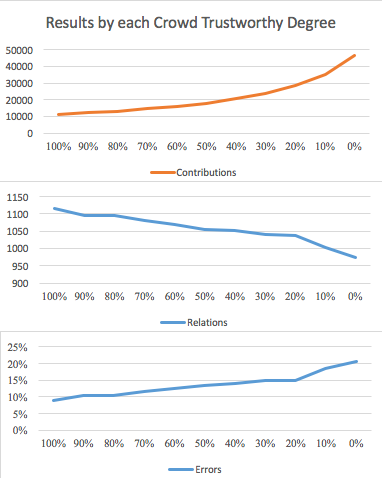
\includegraphics[scale=0.8] {figure/results-line}}
	\caption{evolution of results by each between Crowd Trustworthy Degree}
	\label{results-line}
\end{figure}
